%%
%% Template chap1.tex
%%

\chapter{Evaluation of Social Recommendation Systems}

\section{Evaluation Metrics}

\begin{comment}
This paper uses a lot of different evaluation metric to compare the various algorithms discussed. For the collaboration recommendation algorithms which were run the MovieLens dataset, they were solving a regression problem so we used the Root Mean Squared Error (RMSE) metric which was also used to for the Netflix Prize competition.

\[
RMSE = \sqrt{ \frac{\sum_{i=1}^N{ (r_i - p_i)}^2 }{N}}
\]

where {\bf r} are the true rating values for N movies and {\bf p} are the ratings predicted by the recommendation algorithms.

For the social recommendation algorithms, they are trying to solve a classification problem, so instead of RMSE we use various metrics such as accuracy, precision, recall, f1, and a variant of the Mean Average Precision.  Accuracy is a measure of how accurate the algorithm was in classifying all the items.

\[
Accuracy =  \frac{TP + TN}{TP + TN + FP + FN}
\]
\end{comment}

We define True Positives (TP) to be the count of relevant items that were returned by the algorithm, False Positives (FP) to be the count of non-relevant items that were returned by the algorithm, True Negatives (TN) to be the count of non-relevant items that weren't returned by the algorithm, and False Negatives (FN) to be the non-relevant items that were returned by the algorithm.

Precision is a measure of what fraction of items returned by the algorithm were actually relevant.

\[
Precision = \frac {TP} {TP + FP}
\]

\begin{comment}
Recall is the measure of what fraction of all relevant items items were actually returned by the algorithm.

\[
Recall = \frac {TP} {TP + FN}
\]

The F1 score is another measure of an algorithms accuracy, and is calculated as a weighted average between precision and recall.

\[
F1 = 2 \times \frac{precision \times recall}{precision + recall}
\]
\end{comment}

For some queries, results are returned as a ranked list. Therefore the position of an item in the list must also be evaluated, not just whether the item is in the returned list or not. A metric that does this is Average Precision, which computes the precision at every position in a ranked sequence of documents. If $k$ is the rank in a sequence of retrieved documents, $n$ is the number of retrieved documents, and $P(k)$ is the precision at cut-off $k$ in the list. $rel(k)$ is an indicator function equalling 1 if the item at position $k$ is a relevant document, and 0 otherwise. The average precision can be calculated as

\[
AveP = \frac{\sum_{k=1}^n(P(k) \times rel(k))}{\text{number of relevant documents}}
\]

The main metric we use in this paper is the mean average precision (MAP) Since we make a recommendation for each user, these recommendations can be viewed as a separate query per user, and evaluate the average precision for each one. Getting the mean of all the average precisions gives us an effective metric for the entire recommendation system.

\[
MAP = \frac{\sum_{q=1}^Q AveP(q)}{Q}
\]

\section{Design Choices}

\subsection{Facebook and LinkR data}

Using the LinkR Facebook application developed for this project, we were able to gather data on 34,245 users and 407,887 links.\footnote{As of October 18, 2011, 12:15am}
Data available on the users are:

\begin{itemize}
\item {Basic user features:  $gender$, $birthday$, $location$, $hometown$.}
\item {Mapping whether users $\x$ and $\z$ are friends.}
\item {Interactions on Facebook between users $\x$ and $\z$.}
\end{itemize}
Data available on the links are:
\begin{itemize}
\item{User who posted the link}
\item{The user on who's wall the link was posted}
\item{User's description of the link}
\item{Link summary from the webpage}
\item{Number of times the link has been liked}
\item{Number of times the link has been shared}
\item{Number of comments posted on the link}
\item{List of users that have 'liked' the link.}
\end{itemize}
Additionally, links that have been recommended by the LinkR application have the following extra features:
\begin{itemize}
\item{List of users who have clicked on the url.}
\item{Optional "Like" or "Dislike" rating of the LinkR user on the link.}
\end{itemize}

We also consider the users who posted the link to have implicitly liked it already. Outside of the "Dislike" ratings that we are able to get from the LinkR data, there is no other functionality within Facebook itself that allows users to explicitly define which link they do not like. Therefore, we need some way to infer disliked links during training. During training we consider links that were posted by the user's friends and which they have not likes as an evidence that they dislike a link. This is actually a big assumption as in a lot of cases given the nature of the Facebook news feed they may simply have not seen the link yet, and may actually like the link if they see it. Nevertheless, we find in our passive experiment and in live trial that this assumption is still useful.

\subsection{Training Data}

Because of the sheer size of the Facebook data, it was impractical to run training and recommendations over the entire dataset. To keep the runtime of our experiments within reason, we used only the most recent 4 weeks of data for training the recommenders. This also helps alleviate some temporal aspects of the user's changing preferences, i.e., what the user liked last year may not be the same as what he or she likes this year. We also distinguish between the three types of link like/dislike data we can get from the dataset:

\begin{itemize}
\item {ACTIVE: The explicit "Like" and "Dislike" rating that an application user gives on a recommended link. In addition to this, a click by a user on a recommended link also counts as a like by that user on that particular link. Only LinkR users have this data.}
\item {PASSIVE: The like data given to us by Facebook through the Graph API, plus the inferred dislikes as detailed above. }
\item{UNION: Combination of the ACTIVE and PASSIVE data.}
\end{itemize}

\subsection{Live Online Recommendations}

For the recommendation made to the LinkR application users,  we select only links posted in the most recent two weeks that the user has not liked. We use only the links from the last two weeks because we consider recency to be a big issue. Older links have a greater chance of being about things that are outdated already, or worse, the URL for the link may be broken and not working anymore. We have settled on recommending three links per day to the LinkR users and according to the survey done at the end of the first trial, three links per day seems to be just the right number.

For the live trials, Facebook users who installed the LinkR application were randomly assigned one of the four algorithms in each of the two trials. Users were not informed which algorithm was assigned to them to remove any bias. We distinguish our recommended links into two major classes, links that were posted by the LinkR user's friends and links that were posted by users other than the LinkR user's friends. The reason for this is we wished to see whether the users would prefer recommended links from friends or from strangers. The LinkR users were encouraged to rate the links that were recommended to them, and even provide feedback comments on the specific links. In turn these ratings became part of the training data for the recommendation algorithms, and thus was used to improve the performance of the algorithms over time. Based on the user feedback, we filtered out non-English links and links without any descriptions from the recommendations to prevent user annoyance.

At the end of the first trial, we conducted a user survey with the LinkR users to find out how satisfied they were with the recommendations they were getting.

\begin{figure}
\centering
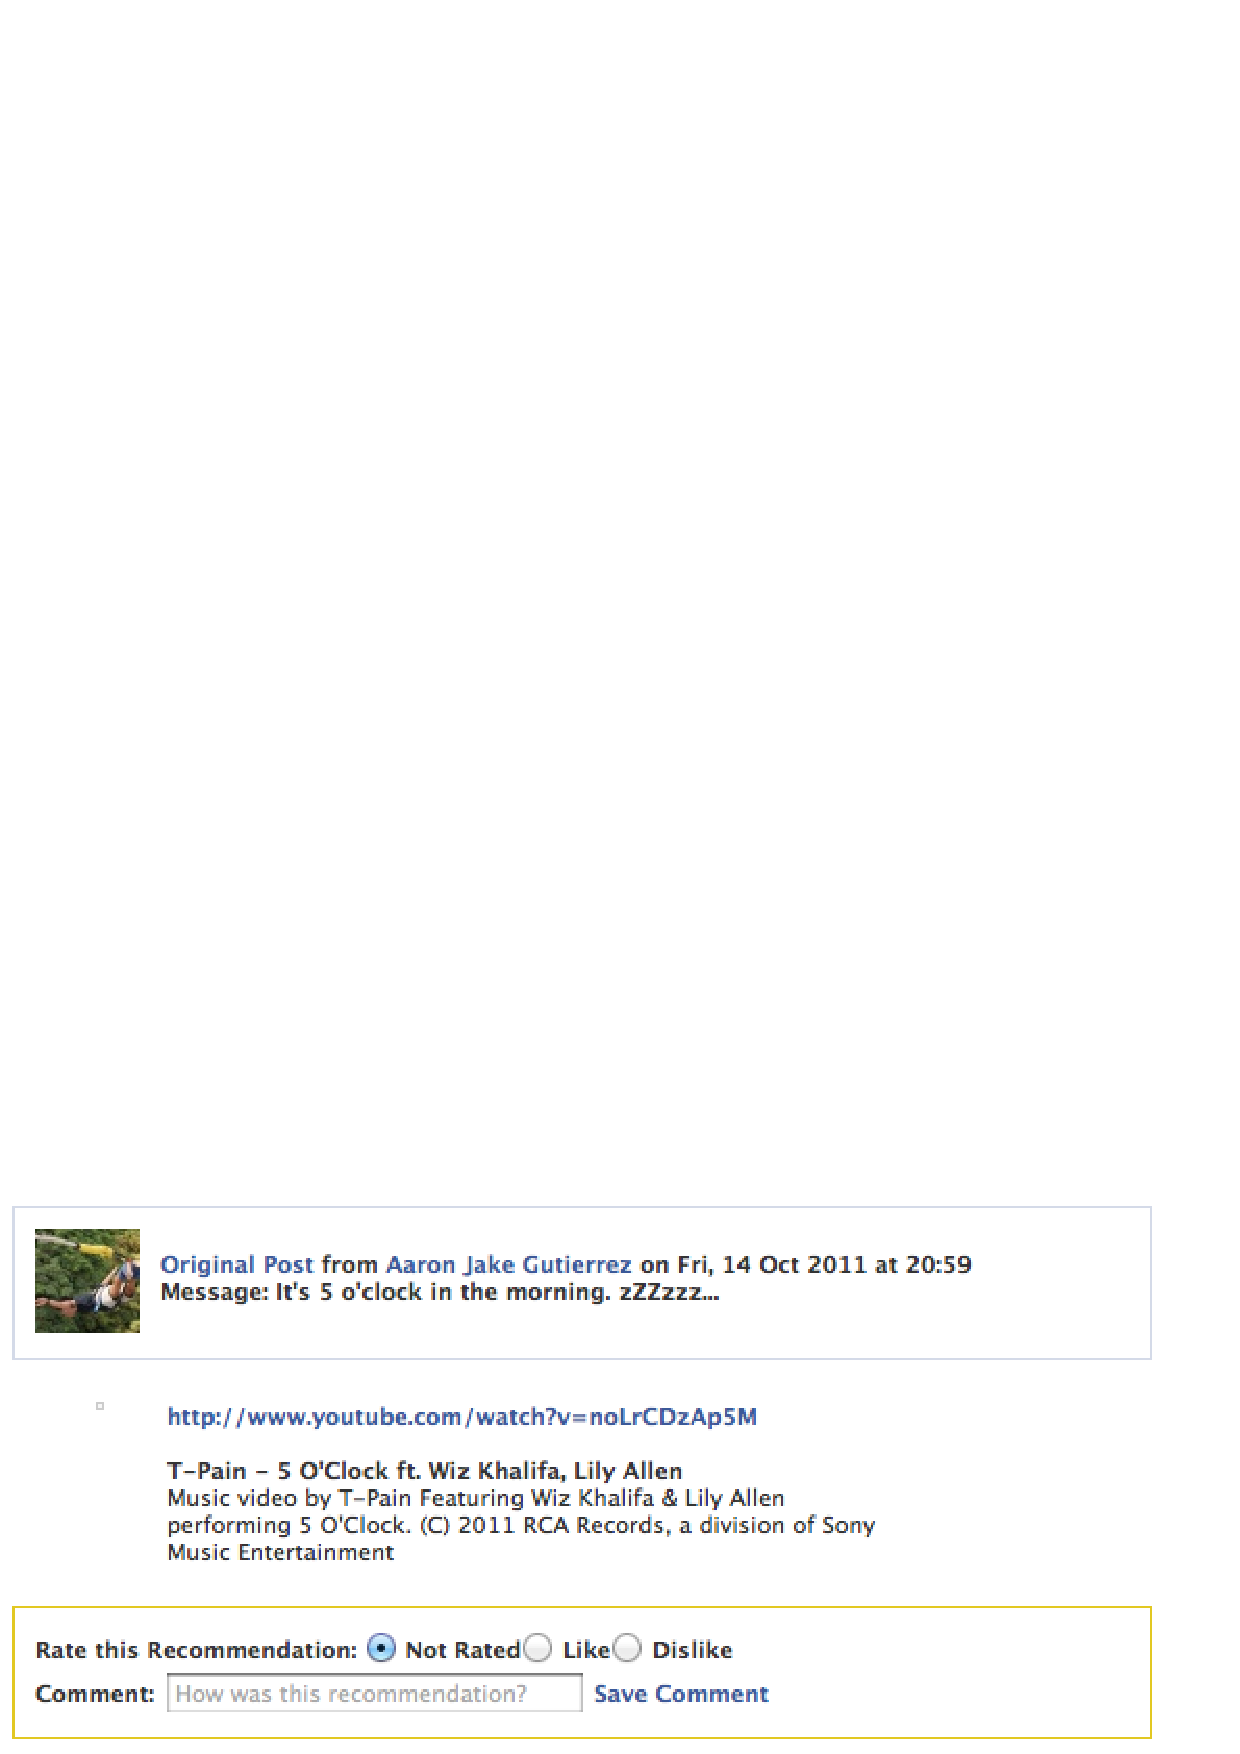
\includegraphics[scale=0.5]{linkr_rating.png}
\caption{Screenshot a LinkR recommendation with the rating and feedback options.}
 \end{figure}
 
\subsection{Test Data}

Our offline testing was used to tune the $\lambda$ parameter values for the various regularizers and for deciding which recommendation algorithms to use in the live trials. Similar to our selection for training data, the test data used for our passive experiment also uses only the most recent 4 weeks of data. We distinguish the test data into the following classes:

\begin{itemize}
\item{FB-USER-PASSIVE: The PASSIVE like/dislike data from all Facebook users in the dataset.}
\item{APP-USER-PASSIVE: The PASSIVE like/dislike data from only the LinkR application users.}
\item{APP-USER-ACTIVE-FRIENDS: The ACTIVE like/dislike data for the LinkR users, but only for friend recommended links.}
\item{APP-USER-ACTIVE-NON-FRIENDS: The ACTIVE like/dislike data for the LinkR users, but only for non-friend recommended links.}
\item{APP-USER-ACTIVE-ALL: The entire active like/dislike data for the LinkR users.}
\end{itemize}

During passive experiments, we simply select which combination of training data and testing data to use. This helped us see which training-test data combination best reflected the results of the live trials Eventually, it was found that using UNION data for training and testing on APP-USER-ACTIVE-ALL best reflected the results of the live trials. 

In cases where training and testing data overlap, i.e., training on PASSIVE and testing on APP-USER-PASSIVE, we get a random 20\% subset of the training data per user for testing. These links are then removed from the training data to ensure that the set of links in the training data and set of links in the test data are disjoint.
